\documentclass{article}
\usepackage[hmargin=3cm, vmargin=3cm]{geometry}
\usepackage{graphicx}
\author{Ben Keller}
\title{Physics 785 Problem Set 2}
\begin{document}
\maketitle
\section{Oxygen Chemical Network}
We can gain a qualitative view of the relative abundances of oxygen compounds
by looking at the reactants needed to produce each species, and the rate
coefficient for the production reactions along with the same information for
reactions that destroy that species.  If a species has numerous reactions
producing it, with relatively high rate coefficeints and abundant precursors,
and few destruction reactions, we can expect to find this compound in abundance
in the molecular ISM. Since many of the compounds in the oxygen chemical network 
are also reactants for producing other compounds, to gain a quantitative estimate, 
integrating the series of coupled differential equations defining the densities
of all species would be necessary.  However, for a number of species (Especially
$H_2$ and $H$, the densities are many orders of magnitude higher than other
compounds, and reactions involving these species will be very rapid, even with
relatively low rate coefficients.  Figure 1 shows graph showing the chemical network
for oxygen.  Reactions that involve additional reactants have their transitions
labeled with the additional reactants, and the transitions are colored based on
the type of reaction involved.  The reaction types and rate coefficients are
defined in the table below:\\

\begin{tabular}{| c | c | c |}
	\hline
	Reaction Type & Rate Coefficient & Colour \\
	\hline
	Neutral-Neutral without Potential Barriers & $10^{-11}$ & Purple\\
	Photodissociation & $10^{-9}$ & Blue\\
	Ion-Molecule Reactions & $10^{-9}$ & Green\\
	Charge Transfer & $10^{-9}$ & Orange\\
	Dissociative Recombination & $10^{-6}-10^{-7}$ & Red\\
	\hline
\end{tabular}\\

The charge transfer rate coefficient was estimated to be on the same order of
magnitude as the coefficients esstimated in Le Teuff et al. 2000.  In addition
to the rate coefficients given above, we also need a rough idea as to the
abundances of some of the precursor compounds.  We know that the abundance of
both atomic and molecular hydrogen is many orders of magnitude higher than all
the other components of the molecular ISM, and so reactions involving those
species will be very efficient.  

From looking at the labeled reaction network,
we can see that the most efficient reactions (Dissociative Recombination) are 
occuring in two production reactions that generate OH, and although it is
involved in a number of reactions that consume it, these reactions all occur
with 2-3 orders of magnitude smaller rate coefficients.  This suggests that OH
is one of the more common species.  The other species involved in dissociative
recombination reactions are CO, which is also created 5 separate reactions (also
suggesting large abundances in the molecular ISM), CO2 (which is formed from the
already established to be abundant OH through a neutral-neutral reaction and
from HCO2+, which due to it's single production reaction from HCO+ is likely not
as abundant as the previous two species), water (which should be produced at a
much lower rate than OH, since its precursor and its super-precursor both will
also form OH), and O2 (which has the largest number of reactions involving it,
and the only rapid dissociation reaction is from a product that must be itself
produced from O2, and so likely is not particularly abundant).  Based on the
network, I would predict that OH, CO, and CO2 are the most most abundant neutral
oxygen species.  Since OH+ is formed from abundant OH transfering charge to H+,
it is also likely to be relatively abundant (although it will rapidly be turned
into H2O+ by reacting with highly abundant H2).  

The species I expect to see in
the lowest abundances are those that have a small number of slow production
reactions coupled with many rapid destruction reactions.  O2H+ is an obvious
example of this, since it is only formed from O2, and rapidly dissociates back
itno O2 and H+.  Another likely rare ion is H3O+ (since it is formed from H2O+ 
which will preferentially form OH, and rapidly is converted into H2O and OH).
\begin{figure}
	\centering
	\includegraphics{oxygen.ps}
	\caption{Chemical network for oxygen species}
\end{figure}\\
\section{Clumps in $\rho$ Ophiuchus}
Johnstone et al. 2000 contains $850 \mu m$ observations of dense 
molecular clumps within the $\rho$ Ophiuchus cloud using the 
SCUBA bolometer on the JCMT.  Using their mass estimates calculated
for a dust temperature of 20K, I generated a differential clump
mass function $\frac{dN}{dM}$, and fit a power law to this distribution
function:
$$\frac{dN}{dM} \propto M^{-\alpha}$$
I first selected only clumps with mass $>0.6M_\odot$.  I chose this selection
firstly because it is greater than the incompleteness limit of $0.4M_\odot$, and
it is the break that Johnstone et al. reports between the two different
power-law slopes of $\alpha=0.5$ (below $0.6M_\odot$) and $\alpha=1.0\pm0.5$
for the cumulative mass function $N(M)$ (this would mean a change in slope for
the differential mass function as well).
I calculated these values by taking a histogram of the base-10 log of the masses
to find the number of clumps $N_i$ at a bin $\log M_i$ of width $\delta \log M$.
$\frac{dN}{dM}$ was then calculated simply as:
$$\frac{dN}{dM}(M_i) = \frac{N_i}{M_i}$$
I used the width of the bin $\delta \log M$ and the relative Poisson noise
$\sqrt{N_i^{-1}}$ as my uncertainties in $\log M_i$ and $\log \frac{dN_i}{dM_i}$
I then used a least squares optimizer from the Scipy python library to fit a
power law (linear in logspace) to $\frac{dN}{dM}$ vs. $M$.  I weighted the
error function using the geometric mean of my two uncertainties.
The result of this fit is a power law with $\alpha = 1.9 \pm 0.3$.  This is
exactly what we would expect if the cumulative mass function has a power law
with $\alpha = 1$, since the derivative will reduce $\alpha$ by one.
$$\frac{dN}{dM} \propto M^{-1.9\pm 0.3}$$
This fit, along with the data, is shown in figure 2.
\begin{figure}
	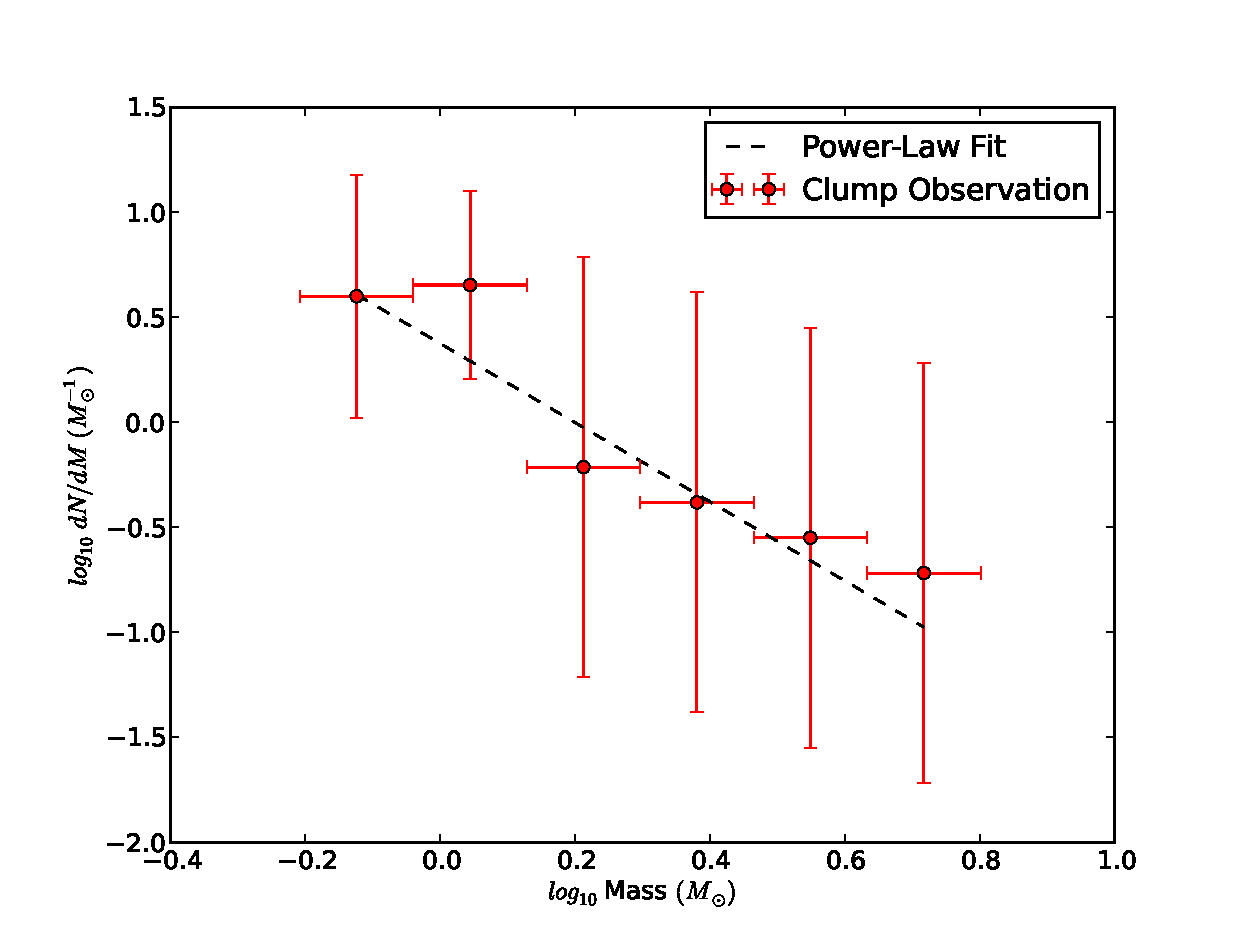
\includegraphics[scale=0.8]{clumpmass.eps}
	\caption{Differential Mass Function dN/dM vs. Clump Mass M}
\end{figure}\\
\textit{Note: All calculations and plots were done using attached code}
\section*{References}
Johnstone et al. 2000 \textit{Large-Area Mapping at 850 Microns. II} ApJ 545,
pp. 327\\
Le Teuff et al. 2000 \textit{The UMIST Database for Astrochemistry 1999} AJS
146, pp. 157\\
\\
\\
\end{document}
